\documentclass[a4paper,10pt]{article}

\usepackage[brazilian]{babel}
\usepackage[left=2.5cm,right=2.5cm,top=3cm,bottom=2.5cm]{geometry}
\usepackage{mathtools}
\usepackage{amsthm}
\usepackage{amsmath}
%\usepackage{nccmath}
\usepackage{amssymb}
\usepackage{amsfonts}
\usepackage{physics}
%\usepackage{dsfont}
%\usepackage{mathrsfs}

\usepackage{titling}
\usepackage{indentfirst}

\usepackage{bm}
\usepackage[dvipsnames]{xcolor}
\usepackage{cancel}

\usepackage{xurl}
\usepackage[colorlinks=true]{hyperref}

\usepackage{float}
\usepackage{graphicx}
%\usepackage{tikz}
\usepackage{caption}
\usepackage{subcaption}

%%%%%%%%%%%%%%%%%%%%%%%%%%%%%%%%%%%%%%%%%%%%%%%%%%%

\newcommand{\eps}{\epsilon}
\newcommand{\vphi}{\varphi}
\newcommand{\cte}{\text{cte}}

\newcommand{\N}{\mathbb{N}}
\newcommand{\Z}{\mathbb{Z}}
\newcommand{\Q}{\mathbb{Q}}
\newcommand{\R}{\vb{R}}
\newcommand{\C}{\mathbb{C}}
\renewcommand{\S}{\hat{S}}
%\renewcommand{\H}{\s{H}}

\renewcommand{\a}{\vb{a}}
\newcommand{\nn}{\hat{n}}
\renewcommand{\d}{\dagger}
\newcommand{\up}{\uparrow}
\newcommand{\down}{\downarrow}

\newcommand{\0}{\vb{0}}
%\newcommand{\1}{\mathds{1}}
\newcommand{\E}{\vb{E}}
\newcommand{\B}{\vb{B}}
\renewcommand{\v}{\vb{v}}
\renewcommand{\r}{\vb{r}}
\renewcommand{\k}{\vb{k}}
\newcommand{\p}{\vb{p}}
\newcommand{\q}{\vb{q}}
\newcommand{\F}{\vb{F}}

\newcommand{\s}{\sigma}
%\newcommand{\prodint}[2]{\left\langle #1 , #2 \right\rangle}
\newcommand{\cc}[1]{\overline{#1}}
\newcommand{\Eval}[3]{\eval{\left( #1 \right)}_{#2}^{#3}}

\newcommand{\unit}[1]{\; \mathrm{#1}}

\newcommand{\n}{\medskip}
\newcommand{\e}{\quad \mathrm{e} \quad}
\newcommand{\ou}{\quad \mathrm{ou} \quad}
\newcommand{\virg}{\, , \;}
\newcommand{\ptodo}{\forall \,}
\renewcommand{\implies}{\; \Rightarrow \;}
%\newcommand{\eqname}[1]{\tag*{#1}} % Tag equation with name

\setlength{\droptitle}{-7em}

\theoremstyle{plain}
\newtheorem{theorem}{Teorema}[section]
%\newtheorem{defi}[theorem]{Definição}
\newtheorem{lemma}[theorem]{Lema}
%\newtheorem{corol}[theorem]{Corolário}
%\newtheorem{prop}[theorem]{Proposição}
%\newtheorem{example}{Exemplo}
%
%\newtheorem{inneraxiom}{Axioma}
%\newenvironment{axioma}[1]
%  {\renewcommand\theinneraxiom{#1}\inneraxiom}
%  {\endinneraxiom}
%
%\newtheorem{innerpostulado}{Postulado}
%\newenvironment{postulado}[1]
%  {\renewcommand\theinnerpostulado{#1}\innerpostulado}
%  {\endinnerpostulado}
%
%\newtheorem{innerexercise}{Exercício}
%\newenvironment{exercise}[1]
%  {\renewcommand\theinnerexercise{#1}\innerexercise}
%  {\endinnerexercise}
%
%\newtheorem{innerthm}{Teorema}
%\newenvironment{teorema}[1]
%  {\renewcommand\theinnerthm{#1}\innerthm}
%  {\endinnerthm}
%
\newtheorem{innerlema}{Lema}
\newenvironment{lema}[1]
  {\renewcommand\theinnerlema{#1}\innerlema}
  {\endinnerlema}
%
%\theoremstyle{remark}
%\newtheorem*{hint}{Dica}
%\newtheorem*{notation}{Notação}
%\newtheorem*{obs}{Observação}


\title{\Huge{\textbf{Lista 4 - Mecânica Estatística}}}
\author{Mateus Marques}

\begin{document}

\maketitle

\section*{1) Gases não ideais}

(a) Primeiramente, como $\displaystyle{N = \ev{\hat{N}} = \frac{\tr[\hat{N} e^{-\beta(\hat{H} - \mu \hat{N})}]}{Z} = \frac{1}{\beta Z} \pdv{Z}{\mu}}$, temos que
$$
\pdvc{N}{\mu}{T,V} = - \frac{\tr[\hat{N} e^{-\beta(\hat{H} - \mu \hat{N})}]}{Z^2} \pdv{Z}{\mu} +
\beta \frac{\tr[\hat{N}^2 e^{-\beta(\hat{H} - \mu \hat{N})}]}{Z} =
$$
$$
= \beta \qty{ \ev{\hat{N}^2} - \ev{\hat{N}}^2 }.
$$


Lembrando que $v = V/N$, temos
$$
\kappa = - \frac{1}{v} \pdvc{v}{P}{T} = - \frac{N}{V} \pdvc{(V/N)}{P}{T,V} =
- \frac{N}{\cancel{V}} \, \cancel{V} \pdvc{(1/N)}{P}{T, V} = -N \qty(-\frac{1}{N^2}) \pdvc{N}{P}{T,V}
$$
$$
= \frac{1}{N} \pdvc{N}{\mu}{T,V} \pdvc{\mu}{P}{T}
$$

Agora de $G(P,T,N) = N \mu(P,T)$, temos
$$
\dd{G} = -S \dd{T} + V \dd{P} + \cancel{\mu \dd{N}} = \cancel{\mu \dd{N}} + N \dd{\mu} \implies
\boxed{ -S \dd{T} + V \dd{P} - N \dd{\mu} = 0. }
$$
Para um processo isotérmico:
$$
V \dd{P} = N \dd{\mu} \implies \pdvc{\mu}{P}{T} = \frac{V}{N}.
$$

Logo
$$
\kappa = \frac{V}{N^2} \pdvc{N}{\mu}{T,V} = \frac{\beta V}{N^2} \, \Big(\ev{\hat{N}}^2 - \ev{\hat{N}^2}\Big).
$$

\n\n\n

(b) Obter $B_2(T)$ e os parâmetros $a$ e $b$ da equação de Van der Waals.

Fatorando a energia livre na parte do gás ideal $F_0$ e na parte de interação, temos
$$
F = - k_B T \qty[
\frac{1}{N!} \int \prod_{i=1}^N \frac{\dd[3]{\r_i} \dd[3]{\p_i}}{(2\pi \hbar)^3} e^{-\beta E(r,p)}
]
$$



(c) Repetir cálculos das notas de aula para o ponto crítico.


\pagebreak

\section*{2) Modelo de Ising de alcance infinito}



\pagebreak

\section*{4) Pontos multicríticos}



\pagebreak

\section*{5) Parâmetros de ordem acoplados}

Temos
$$
f = \frac{1}{2} r_1 m_1^2 + \frac{1}{2} r_2 m_2^2 + u_1 m_1^4 + u_2 m_2^4 + 2 u_{12} m_1^2 m_2^2,
$$
onde $u_1$, $u_2$ e $u_{12}$ são positivos. Defina $\boxed{\Delta = u_1 u_2 - u_{12}^2}$. No item (a) devemos estudar o diagrama de fases para $\Delta > 0$ e no item (b) para $\Delta < 0$.

\n

Pelas definições $r_1 = r - g = a(T-T_1)$ e $r_2 = r+g = a(T-T_2)$, observe que
$$
\begin{cases}
\; g > 0 \iff T_1 > T_2, \\
\; g < 0 \iff T_1 < T_2, \\
\; r_1 < 0 \iff g < r \iff T < T_1, \\
\; r_2 < 0 \iff g > -r \iff T < T_2.
\end{cases}
$$


As fases são caracterizadas por mínimos locais da função $f(m_1, m_2)$. Logo, para estudá-las devemos analisar os pontos em que $\grad{f} = \0$ e que o hessiano de $f$ seja \textit{positivo-definido} (é uma matriz simétrica com autovalores estritamente positivos).

\n

No caso particular de uma matriz simétrica $A$ de dimensão $2 \times 2$, ser positiva-definida significa que
$$
A =
\begin{pmatrix}
A_{11} & A_{12} \\
A_{12}& A_{22}
\end{pmatrix}
, \quad A_{11} > 0, \; A_{22} > 0 \; \text{ e } \det(A) = A_{11} A_{22} - A_{12}^2 > 0.
$$

O gradiente de $f$ é
$$
\grad{f} = \qty(\pdv{f}{m_1}, \pdv{f}{m_2}) =
\qty(r_1 m_1 + 4u_1 m_1^3 + 4u_{12} m_1 m_2^2, \; r_2 m_2 + 4u_2 m_2^3 + 4u_{12} m_2 m_1^2).
$$

Enquanto isso, o hessiano de $f$ é
$$
H_f(x, y) =
\begin{pmatrix}
\pdv[2]{f}{m_1} & \pdv{f}{m_1}{m_2} \\
\pdv{f}{m_2}{m_1} & \pdv[2]{f}{m_2}
\end{pmatrix}
=
\begin{pmatrix}
r_1 + 12 u_1 m_1^2 + 4 u_{12} m_2^2  & 8 u_{12} m_1 m_2 \\
8 u_{12} m_1 m_2 & r_2 + 12 u_2 m_2^2 + 4 u_{12} m_1^2
\end{pmatrix}.
$$


Igualando o gradiente a zero, temos
$$
\boxed{m_1 \Big(
r_1 + 4 u_1 m_1^2 + 4 u_{12} m_2^2
\Big) = 0,}
$$
$$
\boxed{m_2 \Big(
r_2 + 4 u_2 m_2^2 + 4 u_{12} m_1^2
\Big) = 0.}
$$

\n\n\n

As duas equações acima nos dão quatro possibilidades:
\begin{enumerate}
\item $m_1 = m_2 = 0$. Chamaremos esta fase de não-ordenada ($N$). Nela, o hessiano é
$$
H_f(0, 0) =
\begin{pmatrix}
r_1 & 0 \\
0 & r_2
\end{pmatrix}.
$$

Ele é positivo-definido para
$$
r_1 > 0 \e r_2 > 0 \implies \boxed{g < r \e g > -r.}
$$



\item $m_2 = 0$ e $m_1 = m^0_1 = \pm\sqrt{-\frac{r_1}{4 u_1}}$. Chamaremos esta fase de $(F_1)$, onde apenas $m_1 \neq 0$. Devido à raiz quadrada, note que ela só existe caso $r_1 < 0$. Durante a transição, $r_1$ muda de sinal positivo para negativo. Note então que a linha de transição de $(F_1)$ é contínua, já que $m_1 \propto \sqrt{-r_1}$. Calculando o hessiano nesta fase, obtemos
$$
H_f(m_1^0, 0) =
\begin{pmatrix}
-2 r_1 & 0 \\
0 & r_2 - \frac{u_{12}}{u_1} r_1
\end{pmatrix}.
$$

As condições de existência ($m_1$ e $m_2$ serem reais) e estabilidade (o hessiano ser positivo-definido) se traduzem como
$$
r_1 < 0 \e r_2 > \frac{u_{12}}{u_1} r_1
\implies
\boxed{g > r \e g > -\qty(\frac{u_1 - u_{12}}{u_1 + u_{12}}) r. }
$$



\item $m_1 = 0$ e $m_2 = m^0_2 = \pm\sqrt{-\frac{r_2}{4 u_2}}$. Chamaremos esta fase de $(F_2)$, onde apenas $m_2 \neq 0$. Devido à raiz quadrada, note que ela só existe caso $r_2 < 0$. Durante a transição, $r_2$ também muda de sinal positivo para negativo. Note então que a linha de transição de $(F_2)$ é contínua, já que $m_2 \propto \sqrt{-r_2}$. Calculando o hessiano, obtemos
$$
H_f(0, m_2^0) =
\begin{pmatrix}
r_1 - \frac{u_{12}}{u_2} r_2 & 0 \\
0 & -2 r_2
\end{pmatrix}.
$$

As condições de existência e estabilidade se traduzem como
$$
r_2 < 0 \e r_1 > \frac{u_{12}}{u_2} r_2
\implies
\boxed{g < -r \e g < \qty(\frac{u_{2} - u_{12}}{u_2 + u_{12}}) r. }
$$





\item $m_1 \neq 0$ e $m_2 \neq 0$. Chamaremos esta fase de ($F_{12}$). Descobrindo os valores de $m_1$ e $m_2$:
$$
\begin{cases}
\; r_1 + 4 u_1 m_1^2 + 4 u_{12} m_2^2 = 0 \quad [\times (u_{12})] \\
\; r_2 + 4 u_2 m_2^2 + 4 u_{12} m_1^2 = 0 \quad [\times (-u_{1})]
\end{cases}
\implies
\begin{cases}
\; + (u_{12} r_1 + \cancel{4 u_1 u_{12} m_1^2} + 4 u_{12}^2 m_2^2) = 0 \\
\; - (u_1 r_2 + 4 u_1 u_2 m_2^2 + \cancel{4 u_1 u_{12} m_1^2}) = 0
\end{cases}
\implies
$$
$$
(u_{12} r_1 - u_1 r_2) + 4 (u_{12}^2 - u_1 u_2) m_2^2 = 0 \implies
\boxed{ m_2^2 = \gamma_2 = \frac{u_{12} r_1 - u_1 r_2}{4 (u_1 u_2 - u_{12}^2)}, }
$$
e de maneira análoga
$$
\boxed{ m_1^2 = \gamma_1 = \frac{u_{12} r_2 - u_2 r_1}{4 (u_1 u_2 - u_{12}^2)}. }
$$

Perceba que esta fase $(F_{12})$ só existe caso as raízes quadradas sejam reais, ou seja, $\gamma_1 > 0$ e $\gamma_2 > 0$.


Calculando no Mathematica o hessiano da fase $(F_{12})$, temos
$$
H = H_f(\sqrt{\gamma_1}, \sqrt{\gamma_2}) =
\begin{pmatrix}
\frac{2 (u_{12} r_2 - u_2 r_1) u_1}{u_1 u_2 - u_{12}^2} &
2 u_{12} \sqrt{\frac{(u_{12} r_2 - u_2 r_1)(u_{12} r_1 - u_1 r_2))}{(u_{12}^2 - u_1 u_2)^2}} \\
2 u_{12} \sqrt{\frac{(u_{12} r_2 - u_2 r_1)(u_{12} r_1 - u_1 r_2))}{(u_{12}^2 - u_1 u_2)^2}} &
\frac{2 (u_{12} r_1 - u_1 r_2) u_2}{u_1 u_2 - u_{12}^2}
\end{pmatrix}.
$$

A fase $(F_{12})$ é estável se o hessiano $H$ for positivo-definido, ou seja, $H_{11}>0$, $H_{22}>0$ e $\det(H)>0$.

Utilizando as condições de existência e estabilidade da fase $(F_{12})$, a função \texttt{Reduce} do Mathematica simplifica todas as inequações. Eu inseri no Mathematica:
$$
\texttt{Reduce}\qty[\Big\{u_1 > 0, u_2 > 0, u_{12} > 0, \gamma_1 > 0, \gamma_2 > 0,
H_{11} > 0, H_{22} > 0, \det(H) > 0\Big\},
\; \texttt{Reals}].
$$

O Mathematica retornou
$$
\boxed{\Delta = u_1 u_2 - u_{12}^2 > 0}, \quad
r_2 < 0, \quad
r_1 < 0, \quad
r_2 < \frac{u_{12}}{u_1} r_1 \e
r_1 < \frac{u_{12}}{u_2} r_2.
$$

Em particular, isso mostra que a fase $(F_{12})$ só existe para $u_1 u_2 > u_{12}^2$. As condições para $r_1$ e $r_2$ se traduzem nas condições para $r$ e $g$:

$$
\boxed{
g > r, \quad
g < -r, \quad
g < -\qty(\frac{u_1 - u_{12}}{u_1 + u_{12}}) r \e
g > \qty(\frac{u_2 - u_{12}}{u_2 + u_{12}}) r. }
$$

Durante a transição, nós temos que $(u_{12} r_1 - u_1 r_2) \to 0^+$ ou que $(u_{12} r_2 - u_2 r_1) \to 0^+$. Como
$m_1 \propto \sqrt{u_{12} r_2 - u_2 r_1}$ e $m_2 \propto \sqrt{u_{12} r_1 - u_1 r_2}$, temos que as linhas de transição de $(F_{12})$ também são contínuas.


\end{enumerate}

(a) Usando os parâmetros $u_1 = 2$, $u_2 = 2$ e $u_{12} = 1$, que satisfazem a condição $\Delta = u_1 u_2 - u_{12}^2 > 0$ para a fase mista $(F_{12})$ existir, obtemos o seguinte diagrama de fase $r-g$ na Figura \ref{fig:phase_diag-tetra} (graficado no \href{https://www.desmos.com/calculator?lang=pt-BR}{Desmos}, onde inseri todas as inequações obtidas).
\begin{figure}[H]
\centering
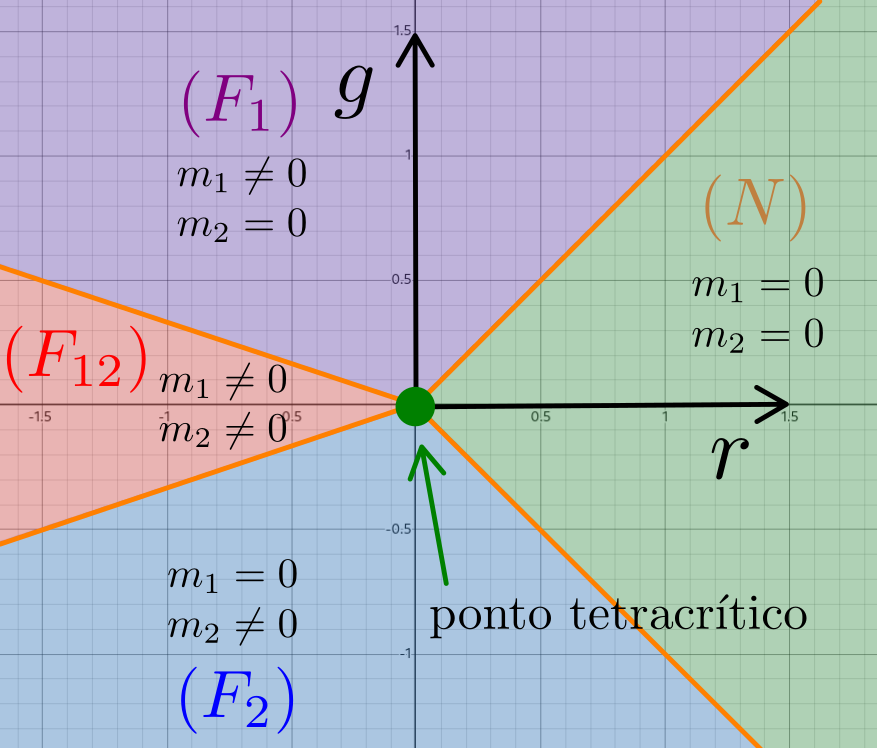
\includegraphics[width=0.4\linewidth]{fig/phase_diag-tetra.png}
\caption{Diagrama de fase para $u_1 = u_2 = 2$ e $u_{12} = 1$, situação em que existe a fase mista $(F_{12})$. As linhas de transição (\textcolor{Orange}{em laranja}) são contínuas e se encontram no ponto tetracrítico $(r = 0, g = 0)$.}
\label{fig:phase_diag-tetra}
\end{figure}

\n\n

(b) Neste item exploraremos o caso $u_1 u_2 < u_{12}^2$. Como fizemos cálculos gerais dos mínimos locais anteriormente, eles também valem aqui. Só que nesse caso a fase mista $(F_{12})$ não existe. As outras três fases $(N)$, $(F_1)$ e $(F_2)$ continuam a existir e são estáveis nas mesmas condições calculadas anteriomente. Se graficarmos o diagrama de fases (para mínimos locais), para os parâmetros $u_1 = 1/2$, $u_2 = 1/2$ e $u_{12} = 1$, obtemos a Figura \ref{fig:phase_diag-tri}.
\begin{figure}[H]
\centering
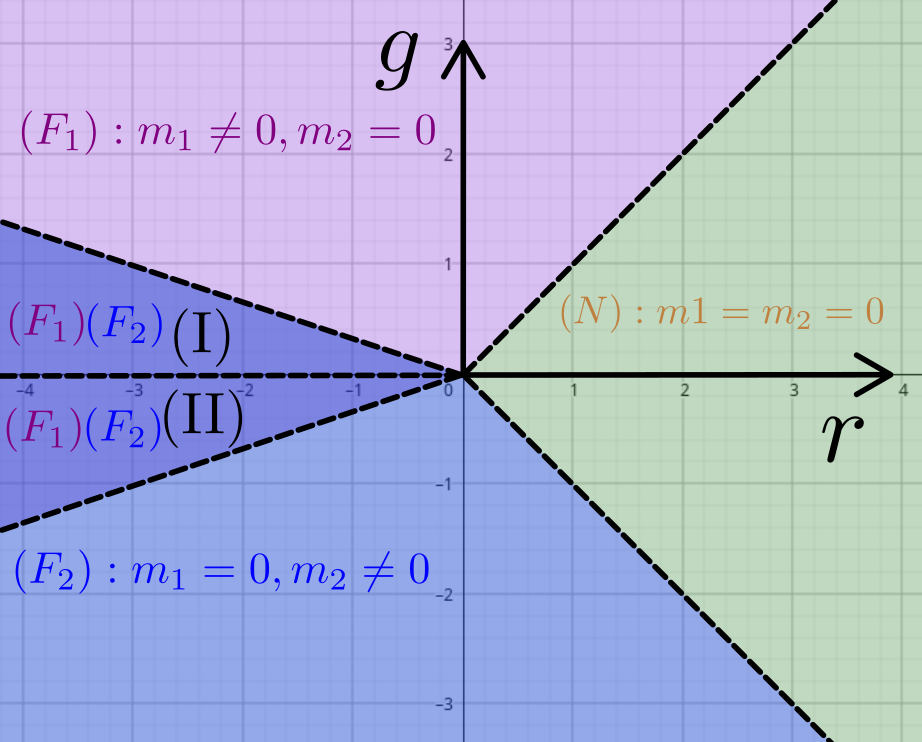
\includegraphics[width=0.4\linewidth]{fig/phase_diag-tri.png}
\caption{Diagrama de fases (mínimos locais) para $u_1 = 0.5$, $u_2 = 0.5$ e $u_{12} = 1$ ($u_1 u_2 < u_{12}^2$). Nesse caso, ambas as fases $(F_1)$ e $(F_2)$ coexistem e são estáveis nas regiões (I) e (II) destacadas à esquerda no gráfico. Mas somente uma delas é o mínimo global.}
\label{fig:phase_diag-tri}
\end{figure}

A explicação para ambas as fases $(F_1)$ e $(F_2)$ coexistirem estavelmente é que ambas se caracterizam como mínimos locais. Para descobrirmos qual fase \textbf{tem preferência}, basta calcularmos qual delas se configura como \textbf{mínimo global}.

\n

Faremos isso comparando $f_1 = f(m_1^0, 0)$ com $f_2 = f(0, m_2^0)$. Temos
$$
f_1 = f(m_1^0, 0) = - \frac{r_1^2}{16 u_1} < 0 \e
f_2 = f(0, m_2^0) = - \frac{r_2^2}{16 u_2} < 0.
$$

Assim, na região (I) da Figura \ref{fig:phase_diag-tri} (que satisfaz as condições $g > 0 \iff r_2 > r_1$ e $r_1 > \frac{u_{12}}{u_2} r_2$), temos
$$
f_1 = - \frac{r_1^2}{16 u_1} < -\frac{u_{12}^2 r_2^2}{16 u_1 u_2^2} = \frac{u_{12}^2}{u_1 u_2}\qty(-\frac{r_2^2}{16 u_2}) = \frac{u_{12}^2}{u_1 u_2} \, f_2 < f_2 \implies \boxed{f_1 < f_2.}
$$

Isso mostra que na região (I) a fase $(F_1)$ tem preferência. Analogamente mostra-se que na região (II) a fase $(F_2)$ tem preferência.

\n

Da mesma forma que no item (a), as transições para a região $(N)$ são contínuas.

\n

Agora, a transição entre as duas fases $(F_1)$ e $(F_2)$ é descontínua, porque mesmo para $r_1$ longe de zero, a fase $(F_1)$ tem $m_1^2 = -\frac{r_1}{4u_1}$, que pula abruptamente para $m_1 = 0$ quando há transição para a fase $(F_2)$. O análogo acontece com $m_2$.

\n


\n\n

O diagrama de fases é então exibido na Figura \ref{fig:phase_diag-bi}.
\begin{figure}[H]
\centering
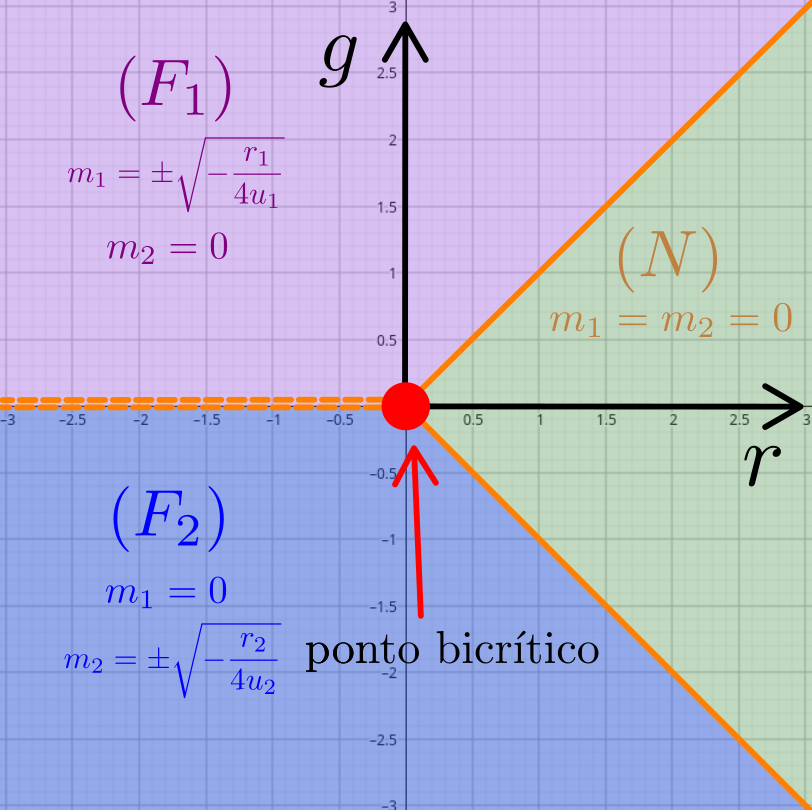
\includegraphics[width=0.6\linewidth]{fig/phase_diag-bi.png}
\caption{Diagrama de fases (mínimos globais) para $u_1 u_2 < u_{12}^2$. As linhas sólidas laranjas são contínuas, enquanto que a linha dupla tracejada laranja configura uma transição descontínua.}
\label{fig:phase_diag-bi}
\end{figure}

\n\n

No caso em que $u_{12} < 0$ e $u_{12}^2 > u_1 u_2$, existem valores de $m_1$ e $m_2$ para os quais a energia livre $f(m_1, m_2)$ decresce indefinidamente. Por exemplo, se $u_1 = 1$, $u_2 = 1$ e $u_{12} = -2$, podemos tomar $m_1 = m_2 = m \to \infty$, de maneira que $f \to -\infty$. Isso se configura como uma região instável, que não faz sentido físico, pois as magnetizações $m_1$ e $m_2$ crescem indefinidamente.


%%%-----
%%% Referências bibliográficas
%%%-----
%\addcontentsline{toc}{chapter}{\bibname}
%%\bibliographystyle{abntex2-num}
%\bibliography{citations}
%\bibliographystyle{ieeetr}


\end{document}
